% !TeX program = pdflatex
% =============================================================================
% Arbeitsblatt: Freier Fall (nicht bewertet, Übungsmaterial für den Unterricht)
% Kantonsschule KFR – Physik, 4. Klasse, 1. HS, Mechanik
%
% Kopiert aus vorlagen/arbeitsblatt-vorlage.tex und um dieselben
% Farb-/Boxdefinitionen ergänzt wie beschleunigung-arbeitsblatt.tex /
% bewegungsgleichungen-arbeitsblatt.tex (gleicher Themencluster, direkt
% anschliessende Lektion). Templates sind selbstständig/nicht DRY, siehe
% CLAUDE.md.
%
% Notation: Wie bewegungsgleichungen-arbeitsblatt.tex wird $x$ statt $s$ für
% den Ort verwendet (direkte Fortsetzung dieser Einheit, siehe
% lernziele.md-Beispielkontext zu LZ1: "aus den bekannten allgemeinen
% Bewegungsgleichungen ... die Fallformeln herleiten"). Koordinatensystem in
% diesem Arbeitsblatt durchgehend "nach oben positiv" (siehe erste
% Theoriebox) -- das ist die in diesem Arbeitsblatt getroffene Wahl, nicht
% die einzig mögliche, siehe Lernschwierigkeit 5 in lernziele.md.
%
% Stand: Lernziele, Einleitung, Theorie und Aufgaben fertig (Reihenfolge =
% Dokumentreihenfolge, siehe Kommentar vor der Lernziele-infobox unten;
% stimmt hier mit der LZ-Nummerierung aus lernziele.md überein, keine
% Umnummerierung nötig).
% =============================================================================
\documentclass[addpoints,11pt,a4paper]{exam}

\usepackage[T1]{fontenc}
\usepackage[utf8]{inputenc}
\usepackage[ngerman]{babel}
\usepackage{lmodern}
\usepackage[a4paper,margin=2.2cm,headheight=14pt]{geometry}
\usepackage{amsmath}
\usepackage{amssymb}
\usepackage{siunitx}
% Hausstil: zusammengesetzte Einheiten immer als echter Bruch (\frac), nicht
% als Schrägstrich inline oder \tfrac. Gilt global für jedes \si/\SI.
\sisetup{per-mode=fraction,fraction-command=\frac}
\usepackage{array,booktabs,tabularx,multirow}
\usepackage{enumitem}
\usepackage{graphicx}
\usepackage{xcolor}
\usepackage{colortbl}
\usepackage{tikz}
\usepackage{physics}
\usepackage{circuitikz}
\usepackage[most]{tcolorbox}
\usepackage{lastpage}
\usepackage{needspace}

\usetikzlibrary{arrows.meta,calc,angles,quotes}

\setlength{\parindent}{0pt}
\setlength{\parskip}{0.45em}

% -----------------------------
% Farben (Hausfarbschema Physik KFR)
% -----------------------------
\definecolor{titleblue}{HTML}{183A6B}
\definecolor{accentblue}{HTML}{2E6F9E}
\definecolor{lightblue}{HTML}{EAF4FB}
\definecolor{verylightblue}{HTML}{F7FBFE}
\definecolor{lightgray}{HTML}{F4F6F8}
\definecolor{darkgray}{HTML}{4A4A4A}
% Für Diagramme mit zwei verschiedenen Funktionen/Linien: titleblue (dunkles
% Blau) + accentorange (Orange) sind weit genug auseinander (auch in
% Graustufen/für Farbenblinde unterscheidbar), im Gegensatz zu
% titleblue+accentblue, die beide Blautöne sind.
\definecolor{accentorange}{HTML}{D9720C}
% Für Diagramme mit DREI Linien: dritte Farbe nötig, die sich sowohl von
% titleblue als auch von accentorange klar unterscheidet, auch in
% Graustufen/für Farbenblinde. Violett liegt weit genug von Blau und Orange
% entfernt, um als dritte Linie eindeutig unterscheidbar zu bleiben.
\definecolor{accentpurple}{HTML}{7B2D8E}
% Theorieblock: eigene Farbe (grün), damit er sich auf einen Blick von den
% blauen Lernziele-/Aufgaben-Boxen abhebt.
\definecolor{theorygreen}{HTML}{2E7D4F}
\definecolor{lighttheorygreen}{HTML}{EAF7EF}
% Gruppenarbeitbox: eigene Farbe (Petrol/Teal), damit Partner-/Gruppenarbeit
% sich auf einen Blick von normalen Einzelaufgaben (blau, taskbox) und vom
% Theorieblock (grün, theoriebox) abhebt. Siehe Regel weiter unten bei
% \newtcolorbox{groupbox}.
\definecolor{groupteal}{HTML}{1B7F72}
\definecolor{lightgroupteal}{HTML}{E8F5F3}

% -----------------------------
% Spaltentypen
% -----------------------------
\newcolumntype{Y}{>{\centering\arraybackslash}X}
\newcolumntype{P}[1]{>{\raggedright\arraybackslash}p{#1}}

% -----------------------------
% Boxen
% -----------------------------
\newtcolorbox{titlebox}{
  enhanced,
  colback=titleblue,
  colframe=titleblue,
  boxrule=0pt,
  arc=3mm,
  left=3mm,right=3mm,top=3mm,bottom=3mm
}

% exam.cls rückt die questions-Liste um die Breite von "10." (plus \labelsep)
% ein (Platz für die Nummerierung "1.", "2." ...); wir messen dieselbe Distanz
% hier unabhängig nach.
\newlength{\aufgabenindent}
\settowidth{\aufgabenindent}{10.\hskip\labelsep}

% left/right-Padding bewusst grosszügiger als bei answerbox: exam.cls hängt
% die Nummerierung von \question bündig an den inneren Rand des
% Textbereichs. Bei zu knappem Padding sitzt diese Nummer direkt auf dem
% Rahmen der Box statt sichtbar innerhalb davon.
% infobox steht ausserhalb von questions (z.B. beim Lernzielblock auf
% Dokumentebene) und braucht deshalb KEINE Korrektur: \linewidth entspricht
% dort bereits \textwidth.
\newtcolorbox{infobox}{
  enhanced,
  breakable,
  colback=lightblue,
  colframe=accentblue,
  boxrule=0.7pt,
  arc=2mm,
  left=5mm,right=5mm,top=2mm,bottom=2mm
}

% theoriebox: wie infobox, aber grün und mit farbigem Titelbalken (analog zu
% taskbox), damit der Theorieblock auf einen Blick von Lernziele (blau,
% ohne Titelbalken) und Aufgaben (blau, mit Titelbalken) unterscheidbar ist.
% Steht wie infobox ausserhalb von questions: KEINE Einrückungskorrektur
% nötig (siehe Kommentar bei infobox oben).
% Regel: hervorgehobene/definierte Begriffe INNERHALB einer theoriebox
% immer mit \textbf{\emph{...}} setzen (fett UND kursiv), nicht mit blossem
% \emph{...}, damit Fachbegriffe beim Durchlesen der Theorie sofort
% auffallen. Ausserhalb von theoriebox (beispielbox, Aufgabentext, ...)
% bleibt \emph{...} allein korrekt.
\newtcolorbox{theoriebox}[1][Theorie]{
  enhanced,
  breakable,
  colback=lighttheorygreen,
  colframe=theorygreen,
  title={#1},
  fonttitle=\bfseries,
  boxrule=0.7pt,
  arc=2mm,
  left=5mm,right=5mm,top=2mm,bottom=2mm
}

% taskbox steht direkt in der questions-Liste (vor dem ersten \question),
% also innerhalb von deren Einrückung. Empirisch (per Pixelvergleich mit der
% Kopfzeilentabelle) verschiebt "enlarge left by" hier die GESAMTE Box
% (nicht nur ihren linken Rand). Ein positiver Wert schiebt sie nach RECHTS,
% nicht nach links, entgegen der naheliegenden Lesart des Schlüsselnamens.
% Ein negativer Wert (-\aufgabenindent) schiebt die Box exakt um die
% Listeneinrückung nach links; width=\textwidth stellt danach wieder die
% volle Breite her, sodass beide Kanten mit der Tabelle übereinstimmen
% (verifiziert per Pixelmessung, Abweichung <=1px @300dpi).
\newtcolorbox{taskbox}[1][]{
  enhanced,
  breakable,
  colback=verylightblue,
  colframe=accentblue,
  title={#1},
  fonttitle=\bfseries,
  boxrule=0.7pt,
  arc=2mm,
  enlarge left by=-\aufgabenindent,
  width=\textwidth,
  left=5mm,right=5mm,top=2mm,bottom=2mm
}

% beispielbox: wie taskbox (blau), aber ausserhalb von questions: deshalb
% wie infobox/theoriebox KEINE Einrückungskorrektur nötig (siehe Kommentar
% bei infobox oben). Für Beispiele in der Theorie: farblich blau wie
% Aufgaben, damit "Beispiel" sich auf einen Blick von der grünen Theorie
% abhebt (Hausstil: grün = Theorie, blau = Beispiele/Aufgaben).
\newtcolorbox{beispielbox}[1][Beispiel]{
  enhanced,
  breakable,
  colback=verylightblue,
  colframe=accentblue,
  title={#1},
  fonttitle=\bfseries,
  boxrule=0.7pt,
  arc=2mm,
  left=5mm,right=5mm,top=2mm,bottom=2mm
}

% Regel für groupbox: JEDE Aufgabe, bei der Schülerinnen/Schüler zu zweit
% oder in einer Gruppe zusammenarbeiten (Partnerarbeit, Gruppenarbeit,
% Diskussion zu zweit, ...), bekommt diese Box statt der blauen taskbox.
% Farbe (Petrol/Teal) ist bewusst weder blau (taskbox/infobox) noch grün
% (theoriebox), damit "hier braucht es eine Partnerin/einen Partner" auf
% einen Blick erkennbar ist. Strukturell identisch zu taskbox (gleiche
% Einrückungskorrektur, da auch groupbox innerhalb von questions steht).
\newtcolorbox{groupbox}[1][Gruppenarbeit]{
  enhanced,
  breakable,
  colback=lightgroupteal,
  colframe=groupteal,
  title={#1},
  fonttitle=\bfseries,
  boxrule=0.7pt,
  arc=2mm,
  enlarge left by=-\aufgabenindent,
  width=\textwidth,
  left=5mm,right=5mm,top=2mm,bottom=2mm
}

% hinweisbox: eigene Farbe (Orange, wiederverwendet accentorange statt einer
% neuen Farbe), für wichtige Klarstellungen, die über eine normale
% Bemerkung im Fliesstext hinausgehen, etwa eine explizite Warnung vor
% einer häufigen Verwechslung. Steht wie infobox/theoriebox/beispielbox
% ausserhalb von questions, KEINE Einrückungskorrektur nötig.
\definecolor{lightorange}{HTML}{FCEEE0}
\newtcolorbox{hinweisbox}[1][Hinweis]{
  enhanced,
  breakable,
  colback=lightorange,
  colframe=accentorange,
  title={#1},
  fonttitle=\bfseries,
  boxrule=0.7pt,
  arc=2mm,
  left=5mm,right=5mm,top=2mm,bottom=2mm
}

% formelbox: eigene Farbe (Violett, wiederverwendet accentpurple), um die
% zentralen Fallformeln dieser Einheit visuell klar von normaler Theorie
% abzuheben, analog zu bewegungsgleichungen-arbeitsblatt.tex. Steht wie
% infobox/theoriebox/beispielbox ausserhalb von questions, KEINE
% Einrückungskorrektur nötig.
\definecolor{lightpurple}{HTML}{F3EAF7}
\newtcolorbox{formelbox}[1][Fallformel]{
  enhanced,
  breakable,
  colback=lightpurple,
  colframe=accentpurple,
  title={#1},
  fonttitle=\bfseries,
  boxrule=0.9pt,
  arc=2mm,
  left=5mm,right=5mm,top=2mm,bottom=2mm
}

\newtcolorbox{answerbox}{
  breakable,
  colback=white,
  colframe=gray!55,
  boxrule=0.5pt,
  arc=1.5mm,
  left=2mm,right=2mm,top=2mm,bottom=2mm
}

% --- Lösungen ein-/ausblenden -----------------------------------------------
% Schülerexemplar (Standard): \noprintanswers
% Lehrer-/Lösungsexemplar:    \printanswers
\noprintanswers
% \printanswers

% --- Punkte bleiben intern, werden aber nicht gedruckt ----------------------
% Arbeitsblätter sind nicht benotet. \question[n]/\part[n] bekommen trotzdem
% eine Punktzahl n, rein als interner Anhaltspunkt, der 1:1 an
% \Antwortraum{n} weitergereicht wird, um die Antwortraumgrösse zu
% bestimmen. \pointformat{} (Aufruf, nicht \renewcommand!) unterdrückt die
% von der exam-Klasse sonst automatisch gedruckte Punktanzeige ("(n P.)")
% vollständig, ohne die interne Punktezählung (\numpoints) zu beeinflussen.
\pointformat{}

% --- Lösungsbox auf Deutsch, farblich abgesetzt -----------------------------
\renewcommand{\solutiontitle}{\noindent\color{titleblue}\textbf{Lösung:}\enspace}

% --- Kopf-/Fusszeile: Thema/Titel oben, Seitenzahl unten --------------------
\pagestyle{headandfoot}
\cfoot{\textcolor{darkgray}{Seite \thepage\ von \pageref{LastPage}}}

% --- Kopfzeile: Klasse / Datum / Thema / Titel ------------------------------
% Einheitliches Layout für Arbeitsblatt, Prüfung und Praktikum. Ohne Tabelle:
% Klasse/Datum/Thema/Lehrperson stehen als einfache Textzeile unter dem
% Titel-Banner.
\newcommand{\Kopfzeile}[4]{%
  \begin{titlebox}
    {\color{white}\sffamily\bfseries\Large #4}
  \end{titlebox}
  \vspace{0.5em}
  \noindent\textbf{Klasse:}~#1 \hfill \textbf{Datum:}~#2 \hfill \textbf{Thema:}~#3
    \hfill \textbf{Lehrperson:}~Loris Keller
  \vspace{0.8em}
  \lhead{\textcolor{darkgray}{#3}}
  \rhead{\textcolor{darkgray}{#4}}
}

% --- Antwortraum: ca. 2.5 cm Platz pro Punkt, als umrandetes Feld -----------
\newlength{\antwortraumlen}
\newcommand{\Antwortraum}[1]{%
  \pgfmathsetlength{\antwortraumlen}{#1*2.5cm}%
  \begin{answerbox}
    \rule{0pt}{\antwortraumlen}%
  \end{answerbox}%
}

% Werte für Kopfzeile zentral setzen
\newcommand{\Klasse}{4a}
\newcommand{\Datum}{18.09.2026}
\newcommand{\Thema}{Freier Fall}
\newcommand{\ArbeitsblattTitel}{Arbeitsblatt: Freier Fall}

\begin{document}

\Kopfzeile{\Klasse}{\Datum}{\Thema}{\ArbeitsblattTitel}

% --- Lernziele: aus lernziele.md (Backward-Design, Stufe 1) übernommen.
% LZ1..LZ6 hier entsprechen der Reihenfolge, in der die zugehörigen
% Theorieboxen/Übungen im Dokument erscheinen; das stimmt hier zufällig mit
% der ursprünglichen Backward-Design-Reihenfolge überein (wie bei
% beschleunigung-arbeitsblatt.tex), keine Umnummerierung nötig.
% Reihenfolge: LZ2 (Massenunabhängigkeit, direkt im Anschluss an die
% Einleitung als Partnerarbeit erlebt) -> LZ1 (Spezialfall a=g formal
% hergeleitet) -> LZ3 (freier Fall aus der Ruhe) -> LZ4 (Wurf nach oben) ->
% LZ5 (Umkehrpunkt, direkt im Anschluss an LZ4, weil er dieselbe Situation
% vertieft) -> LZ6 (Diagramme, als zusammenfassende Synthese ans Ende
% gesetzt).
\begin{infobox}
\textbf{Lernziele}\\
Am Ende dieser Einheit kann ich \dots
\begin{itemize}[leftmargin=1.2cm,itemsep=0.25em]
  \item begründen, weshalb im Modell ohne Luftwiderstand alle Objekte unabhängig von ihrer Masse gleich schnell fallen. (LZ2)
  \item erklären, weshalb freier Fall und senkrechter Wurf ein Spezialfall der bereits bekannten Bewegungsgleichungen mit $a=g$ sind. (LZ1)
  \item für einen freien Fall aus der Ruhe ($v_0=0$) Fallzeit und Fallstrecke berechnen, mit konsistentem Vorzeichen von $g$ relativ zum gewählten Koordinatensystem. (LZ3)
  \item für einen senkrechten Wurf nach oben die Steigzeit, die maximale Höhe und die Gesamtflugzeit berechnen. (LZ4)
  \item begründen, weshalb am höchsten Punkt eines senkrechten Wurfs die Geschwindigkeit null, die Beschleunigung aber weiterhin $g$ ist. (LZ5)
  \item ein qualitatives $x$-$t$-, $v$-$t$- und $a$-$t$-Diagramm für einen freien Fall bzw. senkrechten Wurf skizzieren. (LZ6)
\end{itemize}
\end{infobox}

% --- Einleitung: Apollo-15-Hook, direkt aus lernziele.md übernommen. Kein
% Bild vorhanden, deshalb Text-only (siehe CLAUDE.md: "Bilder werden später
% ergänzt, nicht blockierend"). Bildvorschlag laut lernziele.md: Standbild
% aus dem NASA-Video oder Vergleichsbild Erde/Mond -- sobald verfügbar in
% Bilder/ ablegen und hier zentriert unter dem Boxtitel einfügen. -----------
\begin{beispielbox}[Einleitung: Hammer und Feder auf dem Mond]
\begin{center}
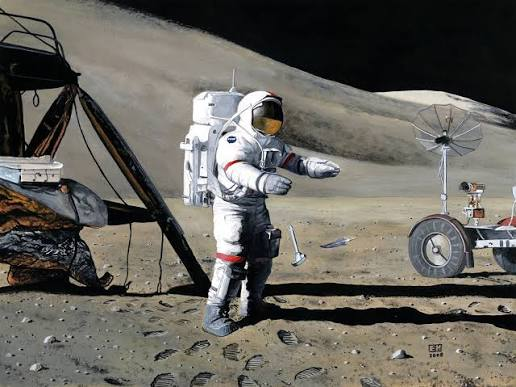
\includegraphics[width=0.6\linewidth]{Bilder/Apollo_15.jpg}
\end{center}
{\scriptsize Illustration des Hammer-Feder-Experiments: David Scott lässt
auf der Mondoberfläche beide Gegenstände gleichzeitig los, im Hintergrund
das Mondfahrzeug (Lunar Roving Vehicle) der Mission Apollo 15.}

Am 2. August 1971 stand der amerikanische Astronaut David Scott während
der Mission Apollo 15 auf der Mondoberfläche, einen Hammer in der einen
und eine Vogelfeder in der anderen Hand. Er liess beide gleichzeitig aus
derselben Höhe los, vor laufender Kamera. Das Ergebnis überraschte viele,
die es zum ersten Mal sahen: Hammer und Feder landeten exakt zur
gleichen Zeit auf dem Boden.

Auf der Erde wäre das undenkbar: Lässt du hier einen Hammer und eine
Feder gleichzeitig los, fällt der Hammer sichtbar schneller. Der
entscheidende Unterschied ist die fehlende Atmosphäre auf dem Mond: Ohne
Luft gibt es auch keinen Luftwiderstand, der die leichte Feder abbremst.
Im idealisierten Modell \glqq freier Fall ohne Luftwiderstand\grqq{}, das
wir in dieser Einheit verwenden, fallen deshalb alle Objekte unabhängig
von ihrer Masse exakt gleich schnell, egal ob Hammer, Feder oder
Mondgestein.

Ein zweiter Unterschied zum Mond kommt dazu: Die Mondgravitation ist
mit $g_{\text{Mond}}\approx\SI{1.62}{\meter\per\second\squared}$ nur
etwa ein Sechstel der Erdbeschleunigung
$g_{\text{Erde}}\approx\SI{9.81}{\meter\per\second\squared}$, die du
bereits aus der Einheit zur Beschleunigung kennst: $g$ ist ein Vektor,
dessen Betrag mit der Distanz zum Erdmittelpunkt abnimmt. Auf
dem Mond fallen Hammer und Feder deshalb zusätzlich viel langsamer als
auf der Erde, obwohl beide Effekte, gleiche Fallzeit unabhängig von der
Masse und geringere Fallbeschleunigung, unabhängig voneinander sind.

Schon rund 350 Jahre vor Apollo 15 hatte Galileo Galilei, der
Namensgeber der \glqq Physik Galileis\grqq{} (dem Themenbereich, in dem
sich auch dieses Arbeitsblatt befindet), genau diese Idee mit einfachen
Mitteln untersucht: Er liess unterschiedlich schwere Kugeln eine schiefe
Ebene hinunterrollen, um die Fallbewegung zu verlangsamen und mit den
Uhren seiner Zeit überhaupt messbar zu machen.

\begin{center}
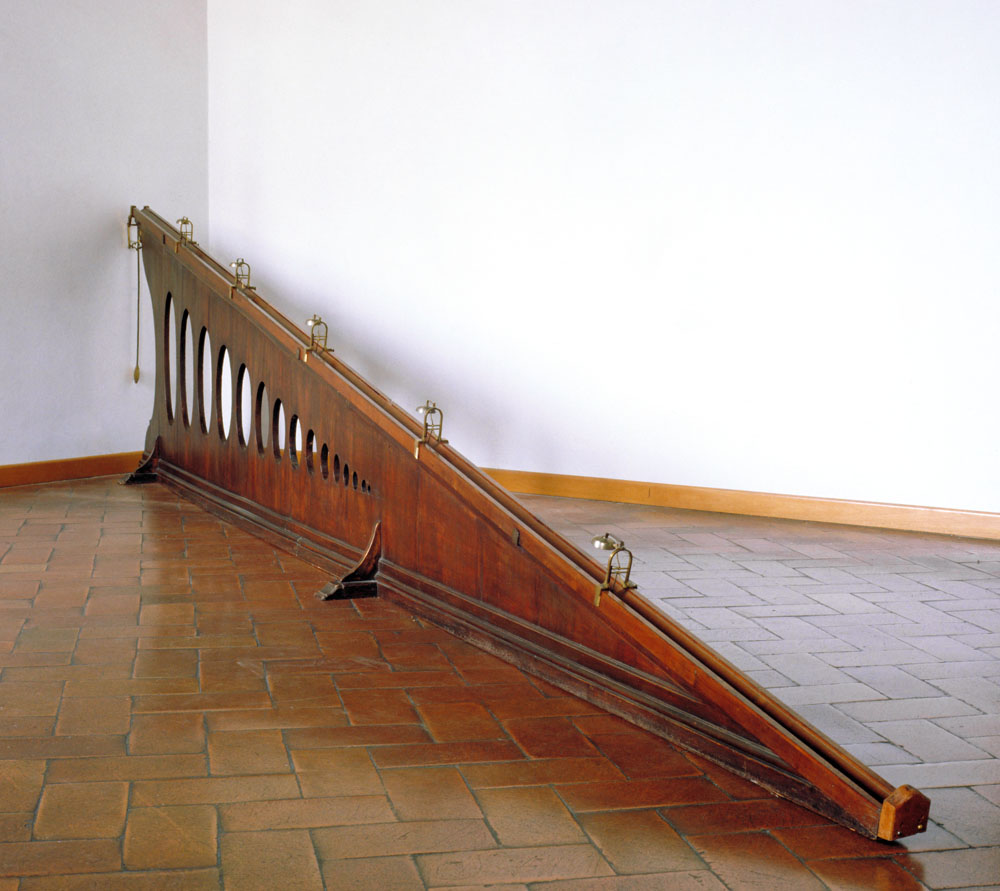
\includegraphics[width=0.55\linewidth]{Bilder/Schiefe_Ebene_Galilei.jpg}
\end{center}
{\scriptsize Nachbau von Galileo Galileis schiefer Ebene, mit der er im
17. Jahrhundert Fallbewegungen untersuchte.}

Seine Schlussfolgerung, dass die Masse eines Körpers seine Fallzeit
nicht beeinflusst, wurde über drei Jahrhunderte später auf dem Mond
eindrücklich bestätigt.
\end{beispielbox}

% --- Partnerarbeit: Predict-Observe-Explain-Münzenexperiment für LZ2,
% direkt im Anschluss an den Hook, wie in lernziele.md vorgeschlagen
% (Beispielkontext "Hook-Fortsetzung"). Adressiert Lernschwierigkeit 1
% (Aristotelisches Fehlkonzept) und 4 (Skepsis ggü. dem Modell). ------------
\begin{groupbox}[Partnerarbeit: Münzenexperiment]
Ihr braucht zu zweit zwei unterschiedlich schwere Gegenstände, zum
Beispiel eine 5-Rappen- und eine 2-Franken-Münze, oder ein
Blatt Papier und einen Radiergummi.

\begin{parts}
  \part[2] \textbf{Predict:} Notiert zuerst, ohne es auszuprobieren, eure
  Vorhersage: Welcher der beiden Gegenstände kommt zuerst am Boden an,
  wenn ihr beide aus derselben Höhe gleichzeitig loslasst? Begründet kurz.
  \Antwortraum{2}

  \part[1] \textbf{Observe:} Lasst beide Gegenstände mehrmals gleichzeitig
  aus derselben Höhe fallen (am besten aus etwa Schulterhöhe, damit ihr
  den Unterschied gut seht). Was beobachtet ihr?
  \Antwortraum{1}

  \part[3] \textbf{Explain:} Stimmt eure Beobachtung mit eurer Vorhersage
  überein? Wiederholt den Versuch danach mit zwei \emph{gleich schweren,
  aber unterschiedlich geformten} Blättern Papier (eines flach, eines zu
  einer Kugel zerknüllt). Woran liegt der Unterschied zwischen den beiden
  Versuchen wirklich: an der Masse oder an etwas anderem?
  \Antwortraum{3}
  \begin{solution}
  Flaches Papier und Radiergummi/Münze fallen unterschiedlich schnell,
  aber \textbf{nicht} wegen ihrer unterschiedlichen Masse, sondern weil
  der Luftwiderstand auf die grosse, leichte Papierfläche viel stärker
  wirkt als auf den kompakten, schweren Gegenstand. Das zeigt der zweite
  Versuch besonders deutlich: Zerknülltes Papier hat exakt dieselbe Masse
  wie das flache Blatt, bietet der Luft aber viel weniger Angriffsfläche
  und fällt deshalb merklich schneller, fast so schnell wie der
  Radiergummi. Im idealisierten Modell \emph{ohne} Luftwiderstand (wie im
  Apollo-15-Experiment auf dem Mond) würde auch das flache Blatt exakt
  gleich schnell fallen wie der Radiergummi.
  \end{solution}
\end{parts}
\end{groupbox}

% =============================================================================
% Theorie: fachliche Grundlage für die Aufgaben, in eigene Boxen unterteilt
% (je Unterthema eine theoriebox), Reihenfolge = Lernzielreihenfolge oben.
% =============================================================================
\begin{theoriebox}[Freier Fall und Wurf: Spezialfall der Bewegungsgleichungen]
Aus der Einheit zu den Bewegungsgleichungen kennst du bereits die drei
allgemeinen Gleichungen für eine gleichmässig beschleunigte Bewegung:
\[
  v(t) = v_0 + a(t-t_0), \qquad
  x(t) = x_0 + v_0(t-t_0) + \frac{1}{2}a(t-t_0)^2, \qquad
  v^2 = v_0^2 + 2a\,\Delta x.
\]
Einheit von $v,v_0\colon\ \si{\meter\per\second}$, von
$x,x_0,\Delta x\colon\ \si{\meter}$, von $t,t_0\colon\ \si{\second}$, von
$a\colon\ \si{\meter\per\second\squared}$.

Ein \textbf{\emph{freier Fall}} (aus der Ruhe, $v_0=0$) und ein
\textbf{\emph{senkrechter Wurf nach oben}} ($v_0\neq0$) sind, solange man
den Luftwiderstand vernachlässigt (idealisiertes Modell), nichts anderes
als Bewegungen mit einer ganz bestimmten, konstanten Beschleunigung: der
bereits bekannten \textbf{\emph{Erdbeschleunigung}} $g\approx
\SI{9.81}{\meter\per\second\squared}$. Man muss also nur $a=g$ (mit dem
richtigen Vorzeichen) in die drei bekannten Gleichungen einsetzen, keine
neue Herleitung nötig.

\textbf{Vorzeichen von $g$:} Die Erdbeschleunigung als Vektor zeigt immer
nach unten (Richtung Erdmittelpunkt), unabhängig davon, ob ein Objekt
gerade fällt oder nach oben fliegt. Das Vorzeichen von $a$ hängt deshalb
davon ab, welche Richtung du für dein Koordinatensystem als positiv
festlegst. \textbf{In diesem Arbeitsblatt gilt durchgehend: nach oben
positiv.} Damit zeigt $g$ (Betrag, immer positiv) in die negative
Richtung, also
\[
  \boxed{a = -g}, \qquad g\approx\SI{9.81}{\meter\per\second\squared}\ \text{(Betrag der Erdbeschleunigung)}.
\]
Eingesetzt in die drei allgemeinen Gleichungen:
\[
  v(t) = v_0 - g(t-t_0), \qquad
  x(t) = x_0 + v_0(t-t_0) - \frac{1}{2}g(t-t_0)^2, \qquad
  v^2 = v_0^2 - 2g\,\Delta x.
\]
\end{theoriebox}

\begin{hinweisbox}
\glqq Nach oben positiv\grqq{} ist in diesem Arbeitsblatt reine
\textbf{\emph{Konvention}}, keine physikalische Notwendigkeit: Genauso
gut könntest du \glqq nach unten positiv\grqq{} wählen, dann würde $a=+g$
gelten. Wichtig ist nur, dass du dich innerhalb einer Aufgabe für eine
Richtung entscheidest und konsequent dabei bleibst, gerade weil freier
Fall (Bewegung nach unten) und Wurf nach oben (Startbewegung nach oben)
in derselben Einheit vorkommen und leicht zu Vorzeichenfehlern verleiten.
\end{hinweisbox}

\begin{questions}
\begin{taskbox}[Übung: Spezialfall selbst nachvollziehen]
\question[5] Setze in der allgemeinen Ortsgleichung
$x(t)=x_0+v_0(t-t_0)+\tfrac{1}{2}a(t-t_0)^2$ die Werte $t_0=0$ und $a=-g$
ein und vereinfache. Vergleiche dein Ergebnis mit der Formel für $x(t)$
in der Theoriebox oben.

\begin{parts}
  \part[2] Setze ein und vereinfache.
  \Antwortraum{2}
  \begin{solution}
  \[
    x(t) = x_0 + v_0(t-0) + \frac{1}{2}(-g)(t-0)^2 = x_0 + v_0t - \frac{1}{2}gt^2.
  \]
  Das stimmt mit der Formel in der Theoriebox überein (dort zusätzlich mit
  allgemeinem $t_0$ statt $t_0=0$).
  \end{solution}

  \part[1] Erkläre in eigenen Worten, weshalb diese Vereinfachung
  zulässig ist, freier Fall und Wurf nach oben also wirklich ein
  Spezialfall der allgemeinen Bewegungsgleichungen sind und keine neue
  Physik brauchen.
  \Antwortraum{2}
  \begin{solution}
  Die allgemeinen Bewegungsgleichungen gelten für \emph{jede} konstante
  Beschleunigung $a$, egal welchen Wert sie hat. Beim freien Fall und
  beim Wurf nach oben ist die Beschleunigung ebenfalls konstant (solange
  man den Luftwiderstand vernachlässigt), nämlich die Erdbeschleunigung
  $g$. Deshalb muss keine neue Formel hergeleitet werden: Es genügt, die
  bereits bekannte, allgemeingültige Formel mit dem konkreten Wert
  $a=-g$ auszuwerten.
  \end{solution}

  \part[2] Angenommen, du hättest statt \glqq nach oben positiv\grqq{}
  die Konvention \glqq nach unten positiv\grqq{} gewählt. Wie lautet die
  Ortsgleichung dann (statt mit $a=-g$)? Was ändert sich am Ergebnis aus
  Teilaufgabe a), was bleibt gleich?
  \Antwortraum{2}
  \begin{solution}
  Bei \glqq nach unten positiv\grqq{} zeigt $g$ in die \emph{positive}
  Richtung, also $a=+g$ statt $a=-g$:
  \[
    x(t) = x_0 + v_0t + \frac{1}{2}gt^2.
  \]
  Es ändert sich nur das Vorzeichen vor dem quadratischen Term (Plus statt
  Minus). Der Betrag jeder berechneten Grösse (Fallzeit, Fallstrecke,
  Steigzeit, \dots) bleibt exakt gleich, unabhängig von der gewählten
  Konvention: Nur die Vorzeichen in der Formel und die Interpretation
  \glqq positiv/negativ\grqq{} ändern sich.
  \end{solution}
\end{parts}
\end{taskbox}
\end{questions}

\begin{theoriebox}[Freier Fall aus der Ruhe]
Für einen freien Fall aus der Ruhe gilt zusätzlich $v_0=0$. Wählt man
ausserdem den Startpunkt als Ursprung ($x_0=0$, $t_0=0$), vereinfachen
sich die Gleichungen aus der vorigen Theoriebox weiter:
\[
  x(t) = -\frac{1}{2}gt^2, \qquad v(t) = -gt.
\]
Beide Werte sind negativ (bei \glqq nach oben positiv\grqq{}): Das Objekt
befindet sich unterhalb des Startpunkts und bewegt sich nach unten. Für
den Alltag ist es meist praktischer, mit positiven Grössen zu rechnen.
Deshalb definiert man die \textbf{\emph{Fallstrecke}}
$h := -x(t)$ (positive Zahl, die Strecke, die das Objekt bereits
zurückgelegt hat) und den Betrag der Geschwindigkeit $\lvert v(t)\rvert$:
\[
  \boxed{h(t) = \frac{1}{2}gt^2}, \qquad \boxed{\lvert v(t)\rvert = gt},
  \qquad \text{Einheit von } h\colon\ \si{\meter}.
\]

\textbf{Fallzeit aus gegebener Fallstrecke:} Manchmal ist nicht $t$,
sondern $h$ gegeben, und $t$ ist gesucht (zum Beispiel: aus welcher Höhe
wurde losgelassen, wenn der Aufprall nach $\SI{2}{\second}$ erfolgt, oder
umgekehrt). Wir lösen $h=\tfrac{1}{2}gt^2$ nach $t$ auf.

\textbf{Schritt 1:} Mit $2$ multiplizieren:
\[
  2h = gt^2.
\]
\textbf{Schritt 2:} Durch $g$ dividieren:
\[
  t^2 = \frac{2h}{g}.
\]
\textbf{Schritt 3:} Wurzel ziehen (die negative Lösung entfällt, da
$t\geq0$ physikalisch sinnvoll sein muss):
\[
  \boxed{t = \sqrt{\frac{2h}{g}}}.
\]

\begin{beispielbox}[Beispiel: Turmsprung]
Ein Turmspringer lässt sich aus $h=\SI{10}{\meter}$ Höhe frei fallen
(Absprung ohne Anfangsgeschwindigkeit nach unten, $v_0=0$). Wie lange
dauert der Fall, und mit welcher Schnelligkeit trifft er auf dem
Wasser auf?

\textbf{Fallzeit:}
\[
  t = \sqrt{\frac{2h}{g}} = \sqrt{\frac{2\cdot\SI{10}{\meter}}{\SI{9.81}{\meter\per\second\squared}}}
  = \sqrt{\SI{2.04}{\second\squared}} \approx \SI{1.43}{\second}.
\]
\textbf{Aufprallschnelligkeit:}
\[
  \lvert v\rvert = gt = \SI{9.81}{\meter\per\second\squared}\cdot\SI{1.43}{\second} \approx \SI{14.0}{\meter\per\second} \approx \SI{50.6}{\kilo\meter\per\hour}.
\]
Zum Vergleich: Das ist ungefähr die Höchstgeschwindigkeit in einer
Tempo-50-Zone, erreicht allein durch einen Sprung aus $\SI{10}{\meter}$
Höhe.
\end{beispielbox}
\end{theoriebox}

\begin{questions}
\begin{taskbox}[Übung: Freier Fall aus der Ruhe]
\question[6] Ein Stein wird von einer Brücke aus $h=\SI{20}{\meter}$
Höhe über dem Fluss losgelassen (aus der Ruhe, kein Wurf).

\begin{parts}
  \part[3] Berechne die Fallzeit bis zum Aufprall auf dem Wasser.
  \Antwortraum{3}
  \begin{solution}
  \[
    t = \sqrt{\frac{2h}{g}} = \sqrt{\frac{2\cdot\SI{20}{\meter}}{\SI{9.81}{\meter\per\second\squared}}} \approx \sqrt{\SI{4.08}{\second\squared}} \approx \SI{2.02}{\second}.
  \]
  \end{solution}

  \part[3] Berechne die Aufprallschnelligkeit, in $\si{\meter\per\second}$
  und in $\si{\kilo\meter\per\hour}$.
  \Antwortraum{3}
  \begin{solution}
  \[
    \lvert v\rvert = gt = \SI{9.81}{\meter\per\second\squared}\cdot\SI{2.02}{\second} \approx \SI{19.8}{\meter\per\second} \approx \SI{71.4}{\kilo\meter\per\hour}.
  \]
  \end{solution}
\end{parts}

\question[4] Dir fällt ein Schlüsselbund aus der Hand (freier Fall aus
der Ruhe); er ist nach $t=\SI{3}{\second}$ am Boden angekommen. Aus
welcher Höhe ist er gefallen?
\Antwortraum{4}
\begin{solution}
\[
  h = \frac{1}{2}gt^2 = \frac{1}{2}\cdot\SI{9.81}{\meter\per\second\squared}\cdot(\SI{3}{\second})^2 = \frac{1}{2}\cdot\SI{9.81}{\meter\per\second\squared}\cdot\SI{9}{\second\squared} \approx \SI{44.1}{\meter}.
\]
\end{solution}
\end{taskbox}
\end{questions}

\begin{theoriebox}[Senkrechter Wurf nach oben]
Beim senkrechten Wurf nach oben ist $v_0>0$ (nach oben, in unserer
Konvention positiv), aber die Beschleunigung bleibt weiterhin $a=-g$: Sie
ändert sich \textbf{\emph{nicht}}, nur weil sich die Wurfrichtung von der
Bewegungsrichtung unterscheidet. Mit Startpunkt $x_0=0$, $t_0=0$ gilt aus
der ersten Theoriebox:
\[
  v(t) = v_0 - gt, \qquad x(t) = v_0t - \frac{1}{2}gt^2.
\]

\textbf{Steigzeit $t_S$:} die Zeit, bis die Geschwindigkeit null wird
(höchster Punkt der Flugbahn). Wir setzen $v(t_S)=0$:

\textbf{Schritt 1:}
\[
  0 = v_0 - gt_S.
\]
\textbf{Schritt 2:} Nach $t_S$ auflösen:
\[
  \boxed{t_S = \frac{v_0}{g}}, \qquad \text{Einheit von } t_S\colon\ \si{\second}.
\]

\textbf{Maximale Höhe $h_{\max}$:} Wir setzen $t_S$ in $x(t)$ ein.

\textbf{Schritt 1:}
\[
  h_{\max} = x(t_S) = v_0\cdot\frac{v_0}{g} - \frac{1}{2}g\left(\frac{v_0}{g}\right)^2.
\]
\textbf{Schritt 2:} Beide Terme ausmultiplizieren/kürzen
($\frac{1}{2}g\cdot\frac{1}{g^2}=\frac{1}{2g}$):
\[
  h_{\max} = \frac{v_0^2}{g} - \frac{v_0^2}{2g}.
\]
\textbf{Schritt 3:} Auf gemeinsamen Nenner $2g$ bringen und
zusammenfassen:
\[
  h_{\max} = \frac{2v_0^2}{2g} - \frac{v_0^2}{2g} = \frac{v_0^2}{2g}.
\]
\[
  \boxed{h_{\max} = \frac{v_0^2}{2g}}, \qquad \text{Einheit von } h_{\max}\colon\ \si{\meter}.
\]
(Alternative Herleitung: aus $v^2=v_0^2-2g\,\Delta x$ mit $v=0$ an der
Spitze direkt nach $\Delta x=h_{\max}$ auflösen, führt zum selben
Ergebnis.)

\textbf{Gesamtflugzeit $T$:} die Zeit vom Abwurf bis zur Rückkehr auf die
Starthöhe ($x=0$). Aus Symmetriegründen (der Weg nach oben und der Weg
zurück nach unten zur selben Höhe dauern wegen $a=\text{konst.}$ gleich
lang) gilt $T=2t_S$:
\[
  \boxed{T = 2t_S = \frac{2v_0}{g}}, \qquad \text{Einheit von } T\colon\ \si{\second}.
\]

\begin{beispielbox}[Beispiel: Ball nach oben geworfen]
Ein Ball wird mit $v_0=\SI{15}{\meter\per\second}$ senkrecht nach oben
geworfen.

\textbf{Steigzeit:}
\[
  t_S = \frac{v_0}{g} = \frac{\SI{15}{\meter\per\second}}{\SI{9.81}{\meter\per\second\squared}} \approx \SI{1.53}{\second}.
\]
\textbf{Maximale Höhe:}
\[
  h_{\max} = \frac{v_0^2}{2g} = \frac{(\SI{15}{\meter\per\second})^2}{2\cdot\SI{9.81}{\meter\per\second\squared}} = \frac{\SI{225}{\meter\squared\per\second\squared}}{\SI{19.62}{\meter\per\second\squared}} \approx \SI{11.5}{\meter}.
\]
\textbf{Gesamtflugzeit:}
\[
  T = 2t_S \approx 2\cdot\SI{1.53}{\second} \approx \SI{3.06}{\second}.
\]
\end{beispielbox}
\end{theoriebox}

\begin{theoriebox}[Der Umkehrpunkt: v ist null, a nicht]
Am höchsten Punkt eines Wurfs nach oben ist die Geschwindigkeit für einen
Moment $v=0$: Der Ball bewegt sich weder nach oben noch nach unten. Genau
an dieser Stelle passiert häufig ein Denkfehler (siehe die
Clicker-Aufgabe unten): Wenn $v=0$ ist, muss dann nicht auch $a=0$ sein?

\textbf{Nein.} Die Beschleunigung ist am Umkehrpunkt weiterhin
$a=-g\approx-\SI{9.81}{\meter\per\second\squared}$, exakt gleich gross
wie während des gesamten Fluges. Der Grund: $a$ ist nicht davon
abhängig, wie schnell sich das Objekt gerade bewegt, sondern beschreibt,
wie sich $v$ \emph{ändert}. Und genau am Umkehrpunkt ändert sich $v$
weiterhin, und zwar am stärksten: Der Ball war gerade noch positiv
schnell (nach oben) und wird im nächsten Moment negativ schnell (nach
unten). Wäre $a$ dort wirklich null, würde $v$ konstant bei $0$ bleiben,
und der Ball würde für immer in der Luft stehen bleiben, statt wieder
herunterzufallen.

\begin{center}
\begin{tikzpicture}[scale=1.15]
  \draw[->] (-0.3,0) -- (6.5,0) node[right] {\scriptsize $t$};
  \draw[->] (0,-2) -- (0,2.3) node[above] {\scriptsize $v$};
  \draw[thick,titleblue] (0,1.8) -- (6,-1.8);
  \draw[dashed,gray] (3,0) -- (3,-1.8);
  \draw (3,0.1) -- (3,-0.1) node[below] {\scriptsize $t_S$};
  \filldraw[black] (3,0) circle (1.6pt);
  \node[above right] at (3,0) {\scriptsize $v=0$, aber Steigung $=a=-g\neq0$};
\end{tikzpicture}\\[0.2em]
{\scriptsize $v$-$t$-Diagramm eines Wurfs nach oben: Bei $t_S$ schneidet
die Gerade die $t$-Achse ($v=0$), ihre Steigung (also $a$) ändert sich an
dieser Stelle aber nicht.}
\end{center}

Derselbe Zusammenhang gilt ganz allgemein an jedem Umkehrpunkt einer
Wurfbewegung, zum Beispiel bei einem Ball, den eine Jongleurin oder ein
Jongleur senkrecht in die Luft wirft: Auch dort bleibt am höchsten Punkt
der Flugbahn die Beschleunigung $g$ bestehen, obwohl die Geschwindigkeit
für einen Moment null ist.
\end{theoriebox}

\begin{questions}
\begin{taskbox}[Clicker-ConcepTest: Der Umkehrpunkt]
\question[3] Ein Ball wird senkrecht nach oben geworfen. Was gilt am
höchsten Punkt seiner Flugbahn?

\begin{parts}
  \part[3] Kreuze die richtige Aussage an und begründe sie in ein bis
  zwei Sätzen.
  \begin{itemize}[leftmargin=1.2cm,itemsep=0.15em]
    \item[$\square$] A: $v=0$ und $a=0$.
    \item[$\square$] B: $v=0$ und $a\neq0$ (weiterhin $g$).
    \item[$\square$] C: $v\neq0$ und $a=0$.
  \end{itemize}
  \Antwortraum{2}
  \begin{solution}
  Richtig ist \textbf{B}. $v=0$, weil der Ball für diesen einen Moment
  weder steigt noch fällt. Aber $a\neq0$: Die Erdbeschleunigung wirkt
  ununterbrochen auf den Ball, auch genau in diesem Moment, sonst könnte
  er im nächsten Moment nicht wieder anfangen zu fallen. Aussage A ist
  der klassische Denkfehler \glqq $v=0$ bedeutet $a=0$\grqq{}, Aussage C ist
  am Umkehrpunkt selbst falsch, da dort $v$ tatsächlich null ist.
  \end{solution}
\end{parts}
\end{taskbox}
\end{questions}

\begin{questions}
\begin{taskbox}[Übung: Wurf nach oben berechnen]
\question[9] Du wirfst einen Ball mit $v_0=\SI{8}{\meter\per\second}$
senkrecht nach oben.

\begin{parts}
  \part[2] Berechne die Steigzeit $t_S$.
  \Antwortraum{2}
  \begin{solution}
  \[
    t_S = \frac{v_0}{g} = \frac{\SI{8}{\meter\per\second}}{\SI{9.81}{\meter\per\second\squared}} \approx \SI{0.82}{\second}.
  \]
  \end{solution}

  \part[2] Berechne die maximale Höhe $h_{\max}$.
  \Antwortraum{2}
  \begin{solution}
  \[
    h_{\max} = \frac{v_0^2}{2g} = \frac{(\SI{8}{\meter\per\second})^2}{2\cdot\SI{9.81}{\meter\per\second\squared}} \approx \SI{3.26}{\meter}.
  \]
  \end{solution}

  \part[2] Berechne die Gesamtflugzeit $T$ bis der Ball wieder auf
  Wurfhöhe ankommt.
  \Antwortraum{2}
  \begin{solution}
  \[
    T = 2t_S \approx 2\cdot\SI{0.82}{\second} \approx \SI{1.64}{\second}.
  \]
  \end{solution}

  \part[3] Deine Freundin wirft einen zweiten Ball senkrecht nach oben,
  der eine maximale Höhe von $h_{\max}=\SI{5}{\meter}$ erreicht. Bestimme
  ihre Anfangsgeschwindigkeit $v_0$ (löse dazu $h_{\max}=v_0^2/(2g)$ nach
  $v_0$ auf).
  \Antwortraum{3}
  \begin{solution}
  \textbf{Schritt 1:} Mit $2g$ multiplizieren:
  \[
    v_0^2 = 2g\,h_{\max}.
  \]
  \textbf{Schritt 2:} Wurzel ziehen (negative Lösung entfällt, da
  $v_0\geq0$ physikalisch sinnvoll sein muss):
  \[
    v_0 = \sqrt{2g\,h_{\max}} = \sqrt{2\cdot\SI{9.81}{\meter\per\second\squared}\cdot\SI{5}{\meter}} = \sqrt{\SI{98.1}{\meter\squared\per\second\squared}} \approx \SI{9.90}{\meter\per\second}.
  \]
  Ihr Ball wurde also etwas schneller geworfen als deiner.
  \end{solution}
\end{parts}
\end{taskbox}
\end{questions}

\begin{theoriebox}[Diagramme: freier Fall und Wurf im Vergleich]
Wie bei den bereits bekannten Bewegungstypen lassen sich freier Fall und
Wurf nach oben qualitativ in $x$-$t$-, $v$-$t$- und $a$-$t$-Diagrammen
darstellen. In beiden Fällen ist $a=-g$ konstant, deshalb ist das
$a$-$t$-Diagramm in beiden Fällen identisch: eine waagrechte Linie bei
$-g$.

\textbf{\emph{Freier Fall aus der Ruhe}} ($v_0=0$, nach oben positiv, das
Objekt bewegt sich also ins Negative):

\begin{center}
\begin{minipage}{0.30\linewidth}\centering
\begin{tikzpicture}[scale=0.6]
  \draw[->] (-0.3,0) -- (5,0) node[right] {\scriptsize $t$};
  \draw[->] (0,-4) -- (0,0.5) node[above] {\scriptsize $x$};
  \draw[thick,titleblue,domain=0:4.3,samples=60,smooth] plot (\x,{-0.2*\x*\x});
\end{tikzpicture}\\[-0.2em]
{\scriptsize $x$-$t$: fallende Parabel}
\end{minipage}\hfill
\begin{minipage}{0.30\linewidth}\centering
\begin{tikzpicture}[scale=0.6]
  \draw[->] (-0.3,0) -- (5,0) node[right] {\scriptsize $t$};
  \draw[->] (0,-3.8) -- (0,0.5) node[above] {\scriptsize $v$};
  \draw[thick,titleblue] (0,0) -- (4.5,-3.6);
\end{tikzpicture}\\[-0.2em]
{\scriptsize $v$-$t$: fallende Gerade ab $0$}
\end{minipage}\hfill
\begin{minipage}{0.30\linewidth}\centering
\begin{tikzpicture}[scale=0.6]
  \draw[->] (-0.3,0) -- (5,0) node[right] {\scriptsize $t$};
  \draw[->] (0,-3.5) -- (0,1.1) node[above] {\scriptsize $a$};
  \draw[thick,titleblue] (0,-2.4) -- (4.5,-2.4);
\end{tikzpicture}\\[-0.2em]
{\scriptsize $a$-$t$: waagrecht bei $-g$}
\end{minipage}
\end{center}

\textbf{\emph{Senkrechter Wurf nach oben}} ($v_0>0$):

\begin{center}
\begin{minipage}{0.30\linewidth}\centering
\begin{tikzpicture}[scale=0.6]
  \draw[->] (-0.3,0) -- (5,0) node[right] {\scriptsize $t$};
  \draw[->] (0,-0.5) -- (0,4) node[above] {\scriptsize $x$};
  \draw[thick,accentorange,domain=0:4.3,samples=60,smooth] plot (\x,{-0.19*(\x-2.15)*(\x-2.15)+3.3});
  \draw[dashed,gray] (2.15,0) -- (2.15,3.3);
  \draw (2.15,0.15) -- (2.15,-0.15) node[below] {\scriptsize $t_S$};
\end{tikzpicture}\\[-0.2em]
{\scriptsize $x$-$t$: Parabel, Scheitel bei $t_S$}
\end{minipage}\hfill
\begin{minipage}{0.30\linewidth}\centering
\begin{tikzpicture}[scale=0.6]
  \draw[->] (-0.3,0) -- (5,0) node[right] {\scriptsize $t$};
  \draw[->] (0,-2) -- (0,2.3) node[above] {\scriptsize $v$};
  \draw[thick,accentorange] (0,1.8) -- (4.3,-1.8);
  \draw[dashed,gray] (2.15,0) -- (2.15,-1.8);
  \draw (2.15,0.15) -- (2.15,-0.15) node[below] {\scriptsize $t_S$};
\end{tikzpicture}\\[-0.2em]
{\scriptsize $v$-$t$: fallende Gerade, Nullstelle bei $t_S$ (vgl.
Umkehrpunktdiagramm weiter oben)}
\end{minipage}\hfill
\begin{minipage}{0.30\linewidth}\centering
\begin{tikzpicture}[scale=0.6]
  \draw[->] (-0.3,0) -- (5,0) node[right] {\scriptsize $t$};
  \draw[->] (0,-3.5) -- (0,1.1) node[above] {\scriptsize $a$};
  \draw[thick,accentorange] (0,-2.4) -- (4.5,-2.4);
\end{tikzpicture}\\[-0.2em]
{\scriptsize $a$-$t$: waagrecht bei $-g$, identisch zum freien Fall}
\end{minipage}
\end{center}

\textbf{Wichtig:} Obwohl sich das $x$-$t$- und das $v$-$t$-Diagramm
zwischen freiem Fall und Wurf nach oben deutlich unterscheiden (andere
Startwerte, andere Kurvenform am Anfang), ist das $a$-$t$-Diagramm in
beiden Fällen exakt gleich: eine waagrechte Linie bei $-g$, die ganze
Zeit über, auch am Umkehrpunkt des Wurfs.
\end{theoriebox}

\begin{questions}
\begin{taskbox}[Übung: Diagramme skizzieren]
\question[10] Ein Ball wird mit $v_0=\SI{10}{\meter\per\second}$ senkrecht
nach oben geworfen (nach oben positiv, Startpunkt $x_0=0$).

\begin{parts}
  \part[2] Berechne zuerst $t_S$ und $h_{\max}$ für diesen Wurf. Du
  brauchst beide Werte in den folgenden Teilaufgaben, um deine Skizzen zu
  beschriften.
  \Antwortraum{2}
  \begin{solution}
  \[
    t_S = \frac{v_0}{g} = \frac{\SI{10}{\meter\per\second}}{\SI{9.81}{\meter\per\second\squared}} \approx \SI{1.02}{\second},
    \qquad
    h_{\max} = \frac{v_0^2}{2g} = \frac{(\SI{10}{\meter\per\second})^2}{2\cdot\SI{9.81}{\meter\per\second\squared}} \approx \SI{5.10}{\meter}.
  \]
  \end{solution}

  \part[2] Skizziere qualitativ das $x$-$t$-Diagramm für die gesamte
  Flugdauer (bis der Ball wieder bei $x=0$ ankommt). Beschrifte den
  Scheitelpunkt mit den Werten aus a).
  \begin{center}
  \begin{tikzpicture}[scale=0.7]
    \draw[->] (-0.3,0) -- (5,0) node[right] {\scriptsize $t$};
    \draw[->] (0,-0.5) -- (0,3.5) node[above] {\scriptsize $x$};
  \end{tikzpicture}
  \end{center}
  \begin{solution}
  \begin{center}
  \begin{tikzpicture}[scale=0.7]
    \draw[->] (-0.3,0) -- (5,0) node[right] {\scriptsize $t$};
    \draw[->] (0,-0.5) -- (0,3.5) node[above] {\scriptsize $x$};
    \draw[thick,titleblue,domain=0:4.2,samples=60,smooth] plot (\x,{-0.17*(\x-2.1)*(\x-2.1)+3});
    \filldraw[black] (0,0) circle (1.6pt);
    \filldraw[black] (4.2,0) circle (1.6pt);
    \draw[dashed,gray] (2.1,0) -- (2.1,3);
    \draw (2.1,0.15) -- (2.1,-0.15) node[below] {\scriptsize $t_S\approx\SI{1.02}{\second}$};
    \node[left] at (-0.05,3) {\scriptsize $h_{\max}\approx\SI{5.10}{\meter}$};
  \end{tikzpicture}
  \end{center}
  Nach oben geöffnete Anfangssteigung (positiv, weil $v_0>0$), Scheitel
  beim Erreichen der maximalen Höhe, danach symmetrischer Abstieg zurück
  auf $x=0$.
  \end{solution}

  \part[2] Skizziere qualitativ das $v$-$t$-Diagramm für dieselbe
  Flugdauer. Beschrifte den Startwert und die Nullstelle mit den
  passenden Werten.
  \begin{center}
  \begin{tikzpicture}[scale=0.7]
    \draw[->] (-0.3,0) -- (5,0) node[right] {\scriptsize $t$};
    \draw[->] (0,-2) -- (0,2.3) node[above] {\scriptsize $v$};
  \end{tikzpicture}
  \end{center}
  \begin{solution}
  \begin{center}
  \begin{tikzpicture}[scale=0.7]
    \draw[->] (-0.3,0) -- (5,0) node[right] {\scriptsize $t$};
    \draw[->] (0,-2) -- (0,2.3) node[above] {\scriptsize $v$};
    \draw[thick,titleblue] (0,1.8) -- (4.2,-1.8);
    \filldraw[black] (2.1,0) circle (1.6pt);
    \node[left] at (0,1.8) {\scriptsize $v_0=\SI{10}{\meter\per\second}$};
    \draw (2.1,0.15) -- (2.1,-0.15) node[below left,xshift=-0.05cm] {\scriptsize $t_S\approx\SI{1.02}{\second}$};
  \end{tikzpicture}
  \end{center}
  Fallende Gerade von positivem Startwert $v_0$ bis zum gleich grossen
  negativen Endwert, Nullstelle genau bei $t_S$ (halbe Gesamtflugzeit).
  \end{solution}

  \part[1] Skizziere qualitativ das $a$-$t$-Diagramm für denselben Wurf.
  \begin{center}
  \begin{tikzpicture}[scale=0.7]
    \draw[->] (-0.3,0) -- (5,0) node[right] {\scriptsize $t$};
    \draw[->] (0,-3.5) -- (0,1.1) node[above] {\scriptsize $a$};
  \end{tikzpicture}
  \end{center}
  \begin{solution}
  \begin{center}
  \begin{tikzpicture}[scale=0.7]
    \draw[->] (-0.3,0) -- (5,0) node[right] {\scriptsize $t$};
    \draw[->] (0,-3.5) -- (0,1.1) node[above] {\scriptsize $a$};
    \draw[thick,titleblue] (0,-2.4) -- (4.2,-2.4);
  \end{tikzpicture}
  \end{center}
  Waagrechte Linie bei $-g$, ohne jeden Knick, auch nicht am
  Umkehrpunkt: Die Beschleunigung ändert sich während des gesamten Flugs
  nicht.
  \end{solution}

  \part[3] Skizziere zusätzlich, in dasselbe $a$-$t$-Diagramm, die
  Beschleunigung eines freien Falls aus der Ruhe (derselbe Betrag $g$,
  aber ohne Wurf davor). Vergleiche beide Kurven: Was ist gleich, was
  unterscheidet sich? Erkläre in ein bis zwei Sätzen, weshalb sich am
  $a$-$t$-Diagramm auch am Umkehrpunkt des Wurfs nichts ändert.
  \begin{center}
  \begin{tikzpicture}[scale=0.7]
    \draw[->] (-0.3,0) -- (5,0) node[right] {\scriptsize $t$};
    \draw[->] (0,-3.5) -- (0,1.1) node[above] {\scriptsize $a$};
  \end{tikzpicture}
  \end{center}
  \Antwortraum{3}
  \begin{solution}
  \begin{center}
  \begin{tikzpicture}[scale=0.7]
    \draw[->] (-0.3,0) -- (5,0) node[right] {\scriptsize $t$};
    \draw[->] (0,-3.5) -- (0,1.1) node[above] {\scriptsize $a$};
    \draw[thick,titleblue] (0,-2.4) -- (4.2,-2.4) node[midway,below] {\scriptsize Wurf};
    \draw[thick,accentorange,dashed] (0,-2.4) -- (2.5,-2.4) node[midway,above] {\scriptsize freier Fall};
  \end{tikzpicture}
  \end{center}
  Beide Kurven liegen exakt auf derselben waagrechten Linie bei $-g$: Ob
  ein Objekt vorher nach oben geworfen wurde oder direkt aus der Ruhe
  fällt, ändert nichts an der wirkenden Beschleunigung, nur an $v_0$. Der
  einzige Unterschied ist, wie lange die Kurve dauert (freier Fall endet
  früher, sobald das Objekt landet). Am Umkehrpunkt des Wurfs ändert sich
  an dieser Linie nichts, weil $a$ dort beschreibt, wie sich $v$ ändert,
  nicht wie schnell das Objekt gerade ist: Die Erdbeschleunigung wirkt
  ununterbrochen, unabhängig davon, ob $v$ gerade positiv, negativ oder
  für einen Moment null ist (siehe Theoriebox \glqq Der Umkehrpunkt\grqq{}
  weiter oben).
  \end{solution}
\end{parts}
\end{taskbox}
\end{questions}

\end{document}
